\chapter[Okra: The Solution Proposal]{Okra: The Solution Proposal}
\label{cp:okra-solution}

{
\parindent0pt

\section{Core Concept and Functionality}
Okra is a mobile-first, web-enabled platform designed as a comprehensive ecosystem to mitigate PHL. The platform serves three primary user groups:

\begin{description}
    \item[Farmers/Producers:] Can create profiles, list their produce (crop type, quantity, harvest date, location), upload images for AI assessment, set indicative prices, and view market demand.
    
    \item[Buyers] Can search for specific produce based on type, quantity, quality (informed by AI score), and location. They can connect with farmers, negotiate, and arrange purchases. Buyers include wholesalers, retailers, processors, and direct consumers.
    
    \item[Logistics Providers] Can register their services (vehicle type – including refrigerated options, capacity, operational routes, pricing). The platform facilitates matching them with farmers/buyers needing transport.
\end{description}

\subsection{Marketplace Networking}
Farmers and producer groups register on the app to list available produce (crop type, quantity, harvest date). Buyers – including wholesalers, processors, and retailers – can search and place orders by region and crop. By centralizing listings, the app ensures farmers find customers quickly, and buyers can discover sources of fresh produce. This reduces unsold inventory and match supply to demand in real time.

\subsection{Logistics Integration}
The app includes a dashboard for logistics providers (truckers, couriers, cold-chain operators). When a sale is made, the system can automatically offer transport jobs to verified drivers. Users can see available vehicles, rates, and track shipments. For example, a farmer in Kano could schedule a refrigerated truck to deliver tomatoes to Lagos. This ensures reliable transport capacity and route planning, cutting delays that lead to spoilage.

\subsection{AI-Powered Insights}
A novel AI feature uses computer vision to analyze produce quality. Farmers or cooperatives upload smartphone images of their harvest batches. The app’s AI model assesses freshness (e.g. spotting bruises, mold, color) and estimates volume or weight from the images. This accomplishes two goals: (1) It provides an objective quality grade for buyers to see, increasing trust. (2) It forecasts how long the produce will remain saleable. The model improves over time as more labeled images are fed back, refining its predictions.

\subsection{Youth-led Agribusiness Empowerment}
The platform encourages youth entrepreneurship. For example, tech-skilled youth can be trained to help digitize farms (taking images, using the app), to become last-mile delivery drivers, or to manage aggregation hubs. The platform could partner with agricultural colleges or startup incubators to recruit graduates. By framing agriculture as a tech-enabled business, the app draws young people into value chains. In effect, it transforms farming from subsistence into a connected, data-driven marketplace, which is more attractive to the next generation.


\section{Screens}


\begin{figure}[H]
    \centering
    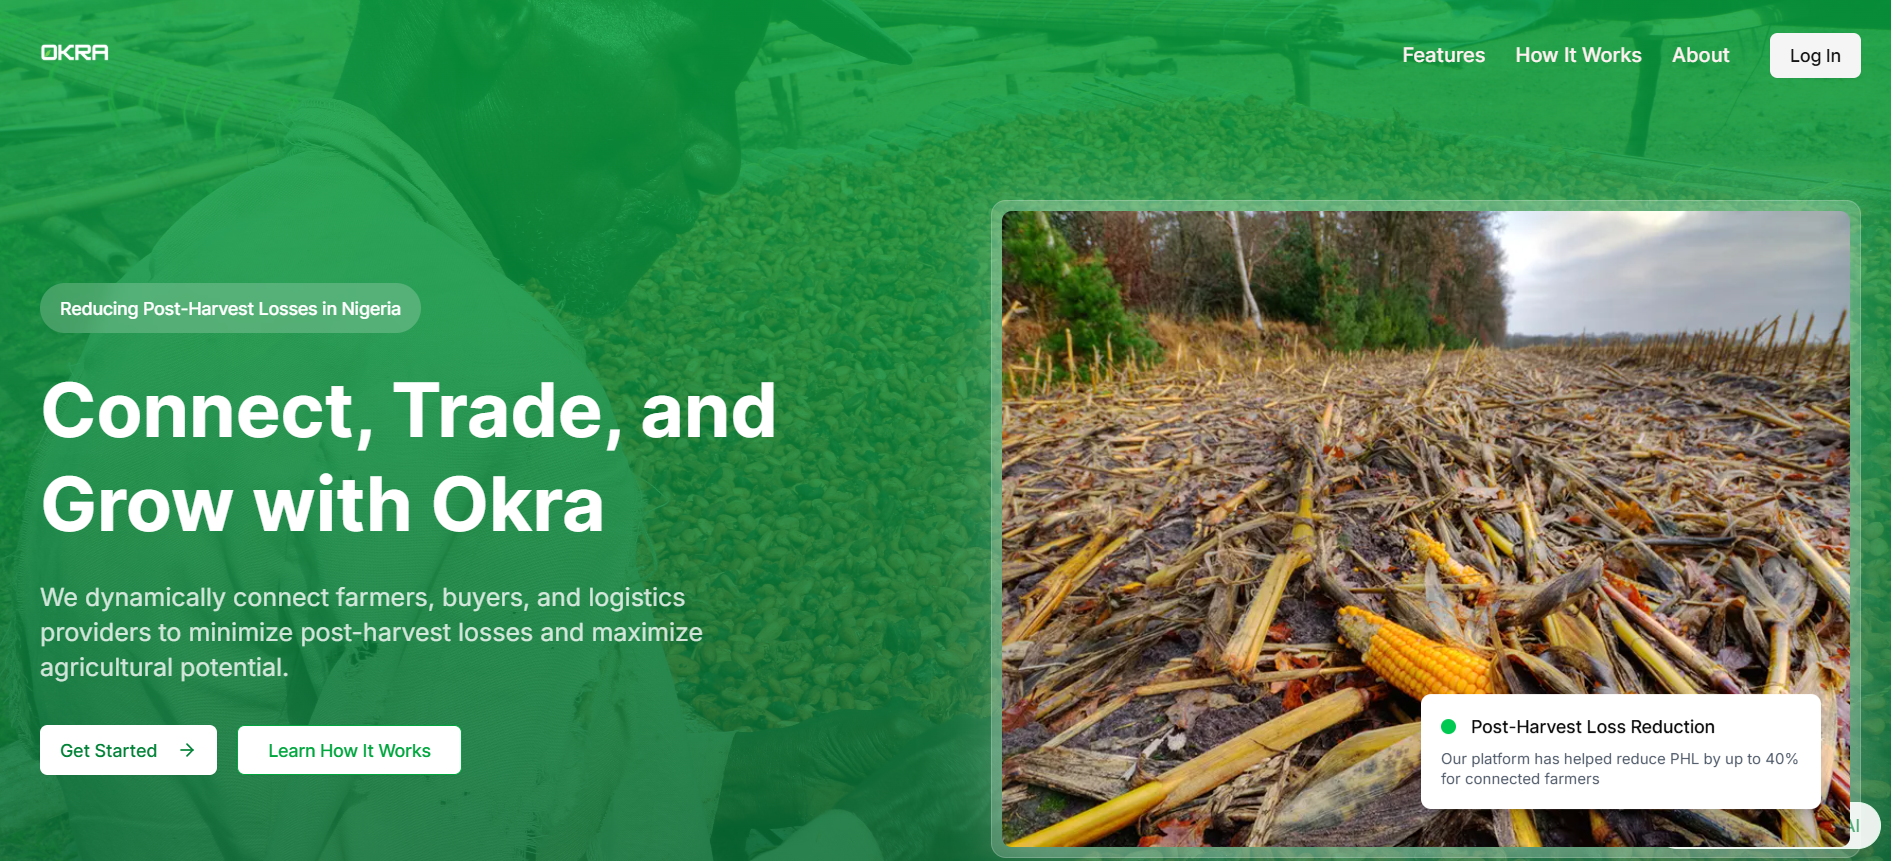
\includegraphics[scale=0.3]{Figures/okra_mockup_landing.png}
    \caption{Screenshot of the landing page}
    \label{fig:figure-05}
\end{figure}


\begin{figure}[H]
    \centering
    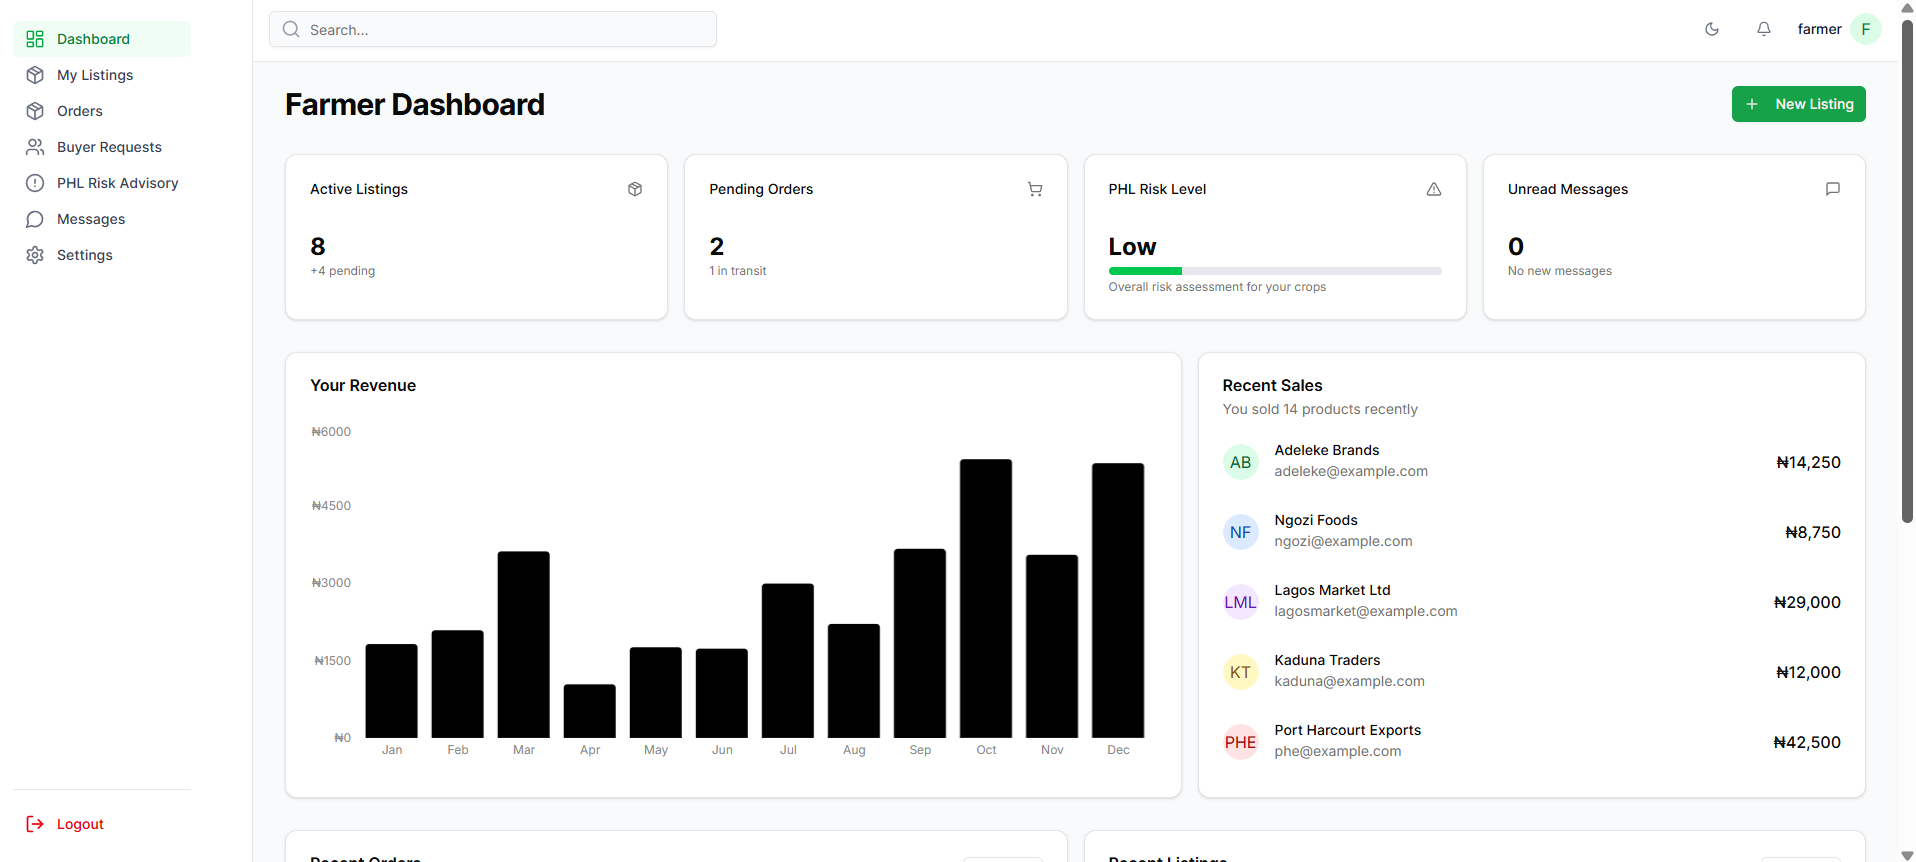
\includegraphics[scale=0.3]{Figures/okra_mockup_farmer_db.png}
    \caption{Screenshot of the farmer's dashboard}
    \label{fig:figure-06}
\end{figure}


\begin{figure}[H]
    \centering
    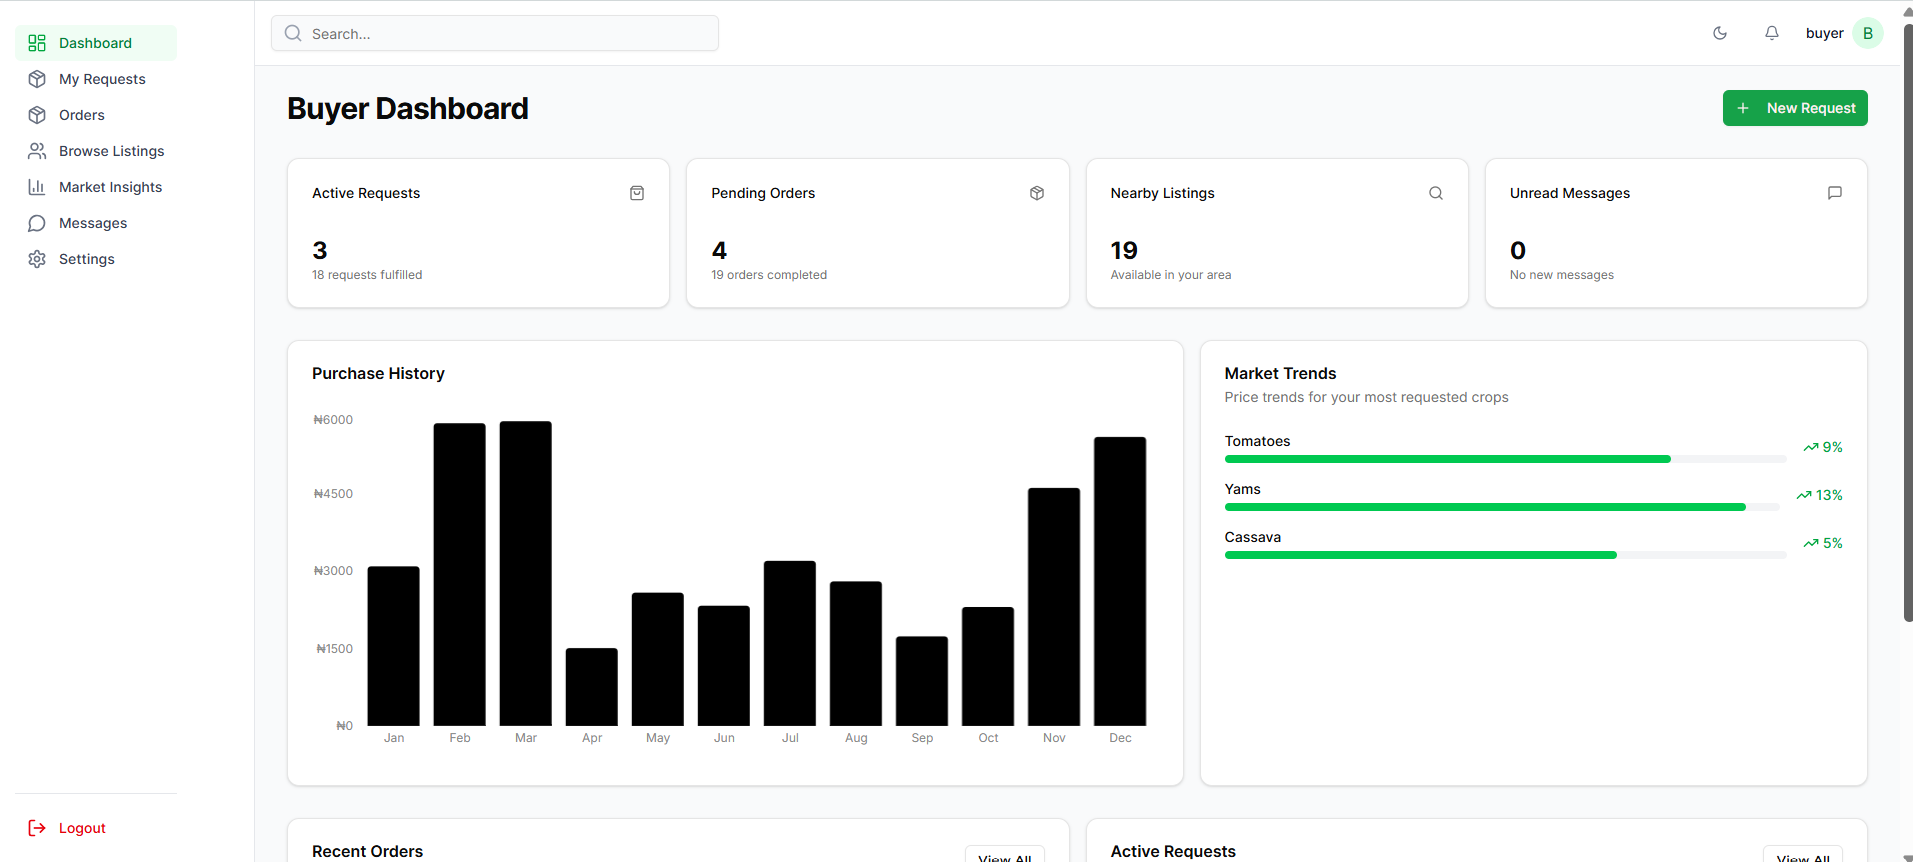
\includegraphics[scale=0.3]{Figures/okra_mockup_buyer_db.png}
    \caption{Screenshot of the buyers's dashboard}
    \label{fig:figure-07}
\end{figure}

\begin{figure}[H]
    \centering
    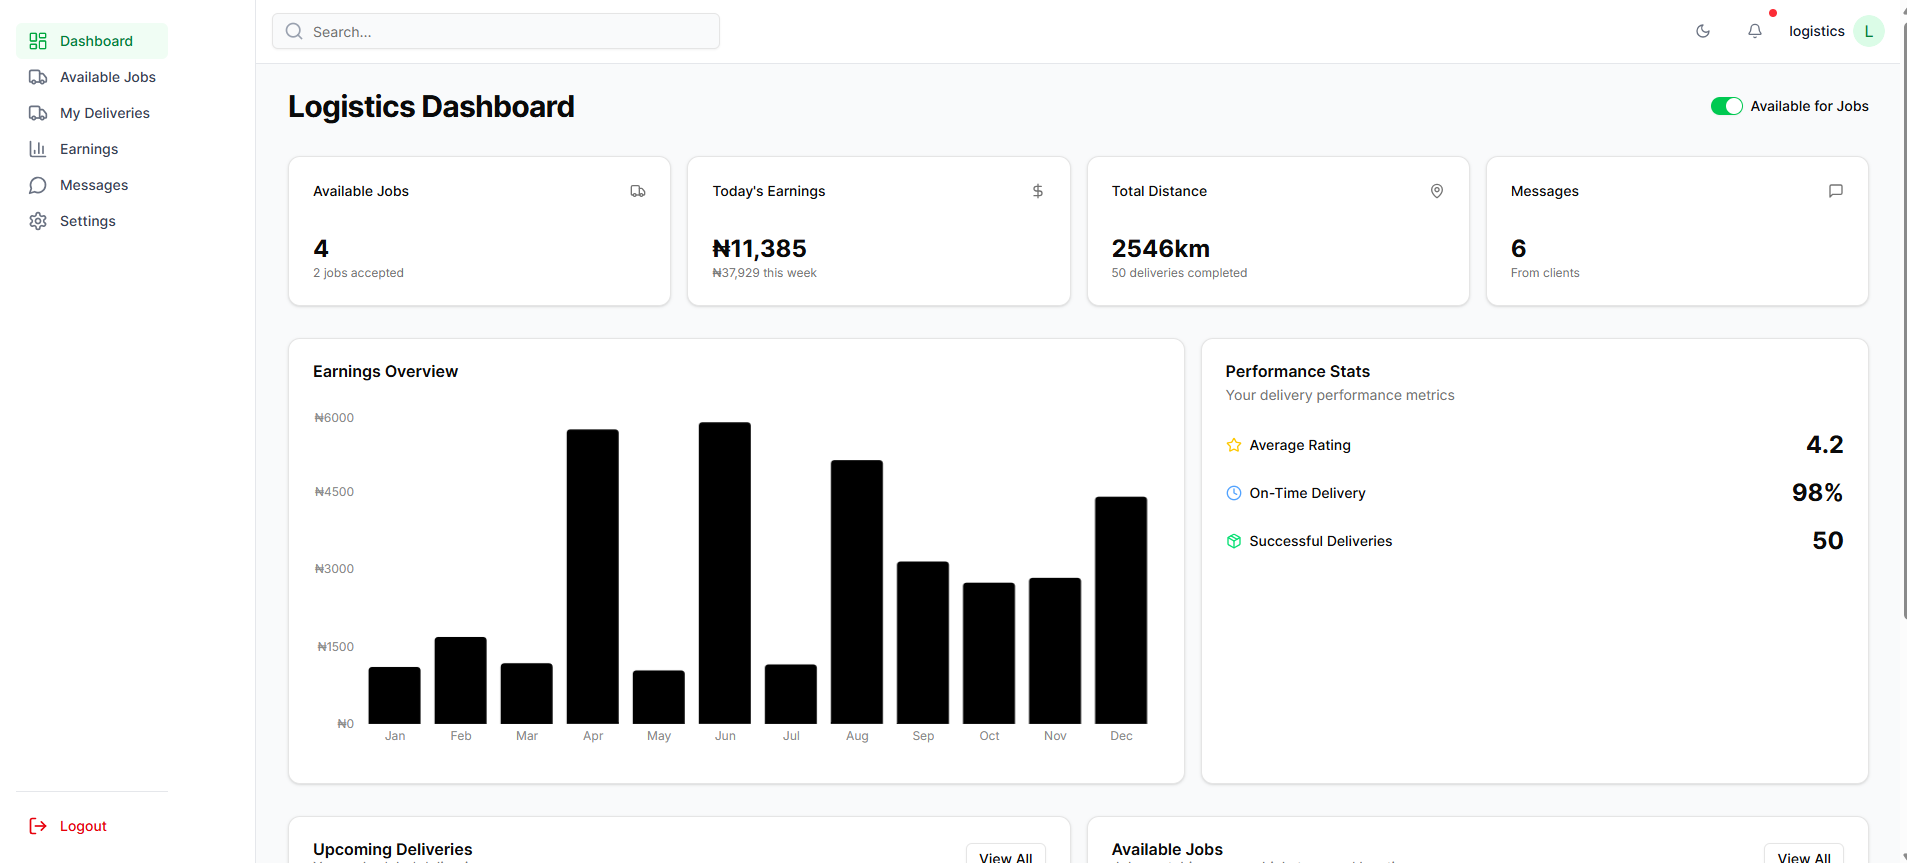
\includegraphics[scale=0.3]{Figures/okra_mockup_logistics_db.png}
    \caption{Screenshot of the buyers's dashboard}
    \label{fig:figure-08}
\end{figure}


\section{Data Strategy}

\subsection{Image Data Collection}
We will collect large numbers of labeled images of harvested produce. This will be done in phases: initially, a pilot program in a few regions (e.g. Kano for tomatoes, Adamawa for maize) will train extension agents and youth volunteers to photograph produce at harvest and at sale. Each image will be tagged with metadata (crop type, variety, region, time, moisture, storage conditions, etc.). Over time, farmers using the app will also upload photos for every batch they list, creating a growing dataset.

\subsection{Data Labeling and Training}
Using expert agronomists and community training, images will be labeled for freshness (e.g. “Fresh”, “Moderately aged”, “Spoiled”) and total count/weight. This labelled dataset feeds the computer vision model. We will employ transfer learning on convolutional neural networks so the AI can accurately assess new images it has not seen before. The initial model will be tested for accuracy and iteratively improved as more data arrives.

\subsection{Feedback Loop (Active Learning)}
Post-deployment, the app will track outcomes of predicted vs. actual. For example, if the AI predicts 10 days of shelf life but spoilage occurs in 7 days, this discrepancy is logged. Buyers and farmers can rate or report the accuracy of freshness ratings. This feedback is used to retrain the model periodically, increasing its accuracy over time. In effect, the app learns from real-world results.

\section{Auxiliary data sources}
In addition to user-generated data, the system will integrate public and commercial datasets for context. Possible sources include:


\begin{description}
    \item[Crop statistics:]  Government or FAO data on regional production volumes and seasonality for major crops.
    
    \item[Geolocation] Maps of farm locations, major roads, market centers.
    
    \item[Weather/Climate] Historical and current weather data per region, since humidity and temperature affect spoilage.
    \item[Market Prices]  Data from local commodity exchanges or market surveys, to show price trends.
    \item[Demographic Data] Farm population and sizes, to profile areas served.This external data enriches the dashboard: for instance, linking rainfall patterns to losses in maize, or highlighting regions that produce a given crop. All data is tied to time and location, enabling spatio-temporal analysis.
\end{description}

\subsection{Privacy and Governance}
Farmers’ personal data (names, exact addresses) will be protected. Only aggregate or anonymized data used on dashboards. Data use agreements will ensure that insights (e.g. “X tonnes of tomatoes sold from Kano”) respect user privacy while guiding decisions.




Geolocation: Maps of farm locations, major roads, market centers.
Weather/Climate: Historical and current weather data per region, since humidity and temperature affect spoilage.
Market Prices: Data from local commodity exchanges or market surveys, to show price trends.
Demographic Data: Farm population and sizes, to profile areas served.
This external data enriches the dashboard: for instance, linking rainfall patterns to losses in maize, or highlighting regions that produce a given crop. All data is tied to time and location, enabling spatio-temporal analysis.
Privacy and Governance: Farmers’ personal data (names, exact addresses) will be protected. Only aggregate or anonymized data used on dashboards. Data use agreements will ensure that insights (e.g. “X tonnes of tomatoes sold from Kano”) respect user privacy while guiding decisions.

}